%!TEX program = xelatex+makeindex+bibtex
\documentclass[final]{scrreprt} %scrreprt of scrartcl
% Include all project wide packages here.
\usepackage{fullpage}
\usepackage{polyglossia}
\setmainlanguage{english}
\usepackage{csquotes}
\usepackage{graphicx}
\usepackage{epstopdf}
\usepackage{pdfpages}
\usepackage{caption}
\usepackage[list=true]{subcaption}
\usepackage{float}
\usepackage{standalone}
\usepackage{import}
\usepackage{tocloft}
\usepackage{wrapfig}
\usepackage{authblk}
\usepackage{array}
\usepackage{booktabs}
\usepackage[toc,page,title,titletoc]{appendix}
\usepackage{xunicode}
\usepackage{fontspec}
\usepackage{pgfplots}
\usepackage{SIunits}
\usepackage{units}
\pgfplotsset{compat=newest}
\pgfplotsset{plot coordinates/math parser=false}
\newlength\figureheight 
\newlength\figurewidth
\usepackage{amsmath}
\usepackage{mathtools}
\usepackage{unicode-math}
\usepackage[
    backend=bibtexu,
	texencoding=utf8,
bibencoding=utf8,
    style=ieee,
    sortlocale=en_US,
    language=auto
]{biblatex}
\usepackage{listings}
\newcommand{\includecode}[3][c]{\lstinputlisting[caption=#2, escapechar=, style=#1]{#3}}
\newcommand{\superscript}[1]{\ensuremath{^{\textrm{#1}}}}
\newcommand{\subscript}[1]{\ensuremath{_{\textrm{#1}}}}


\newcommand{\chapternumber}{\thechapter}
\renewcommand{\appendixname}{Bijlage}
\renewcommand{\appendixtocname}{Bijlagen}
\renewcommand{\appendixpagename}{Bijlagen}

\usepackage[hidelinks]{hyperref} %<--------ALTIJD ALS LAATSTE

\renewcommand{\familydefault}{\sfdefault}

\setmainfont[Ligatures=TeX]{Myriad Pro}
\setmathfont{Asana Math}
\setmonofont{Lucida Console}

\usepackage{titlesec, blindtext, color}
\definecolor{gray75}{gray}{0.75}
\newcommand{\hsp}{\hspace{20pt}}
\titleformat{\chapter}[hang]{\Huge\bfseries}{\chapternumber\hsp\textcolor{gray75}{|}\hsp}{0pt}{\Huge\bfseries}
\renewcommand{\familydefault}{\sfdefault}
\renewcommand{\arraystretch}{1.2}
\setlength\parindent{0pt}

%For code listings
\definecolor{black}{rgb}{0,0,0}
\definecolor{browntags}{rgb}{0.65,0.1,0.1}
\definecolor{bluestrings}{rgb}{0,0,1}
\definecolor{graycomments}{rgb}{0.4,0.4,0.4}
\definecolor{redkeywords}{rgb}{1,0,0}
\definecolor{bluekeywords}{rgb}{0.13,0.13,0.8}
\definecolor{greencomments}{rgb}{0,0.5,0}
\definecolor{redstrings}{rgb}{0.9,0,0}
\definecolor{purpleidentifiers}{rgb}{0.01,0,0.01}


\lstdefinestyle{csharp}{
language=[Sharp]C,
showspaces=false,
showtabs=false,
breaklines=true,
showstringspaces=false,
breakatwhitespace=true,
escapeinside={(*@}{@*)},
columns=fullflexible,
commentstyle=\color{greencomments},
keywordstyle=\color{bluekeywords}\bfseries,
stringstyle=\color{redstrings},
identifierstyle=\color{purpleidentifiers},
basicstyle=\ttfamily\small}

\lstdefinestyle{c}{
language=C,
showspaces=false,
showtabs=false,
breaklines=true,
showstringspaces=false,
breakatwhitespace=true,
escapeinside={(*@}{@*)},
columns=fullflexible,
commentstyle=\color{greencomments},
keywordstyle=\color{bluekeywords}\bfseries,
stringstyle=\color{redstrings},
identifierstyle=\color{purpleidentifiers},
}

\lstdefinestyle{matlab}{
language=Matlab,
showspaces=false,
showtabs=false,
breaklines=true,
showstringspaces=false,
breakatwhitespace=true,
escapeinside={(*@}{@*)},
columns=fullflexible,
commentstyle=\color{greencomments},
keywordstyle=\color{bluekeywords}\bfseries,
stringstyle=\color{redstrings},
identifierstyle=\color{purpleidentifiers}
}

\lstdefinestyle{vhdl}{
language=VHDL,
showspaces=false,
showtabs=false,
breaklines=true,
showstringspaces=false,
breakatwhitespace=true,
escapeinside={(*@}{@*)},
columns=fullflexible,
commentstyle=\color{greencomments},
keywordstyle=\color{bluekeywords}\bfseries,
stringstyle=\color{redstrings},
identifierstyle=\color{purpleidentifiers}
}

\lstdefinestyle{xaml}{
language=XML,
showspaces=false,
showtabs=false,
breaklines=true,
showstringspaces=false,
breakatwhitespace=true,
escapeinside={(*@}{@*)},
columns=fullflexible,
commentstyle=\color{greencomments},
keywordstyle=\color{redkeywords},
stringstyle=\color{bluestrings},
tagstyle=\color{browntags},
morestring=[b]",
  morecomment=[s]{<?}{?>},
  morekeywords={xmlns,version,typex:AsyncRecords,x:Arguments,x:Boolean,x:Byte,x:Char,x:Class,x:ClassAttributes,x:ClassModifier,x:Code,x:ConnectionId,x:Decimal,x:Double,x:FactoryMethod,x:FieldModifier,x:Int16,x:Int32,x:Int64,x:Key,x:Members,x:Name,x:Object,x:Property,x:Shared,x:Single,x:String,x:Subclass,x:SynchronousMode,x:TimeSpan,x:TypeArguments,x:Uid,x:Uri,x:XData,Grid.Column,Grid.ColumnSpan,Click,ClipToBounds,Content,DropDownOpened,FontSize,Foreground,Header,Height,HorizontalAlignment,HorizontalContentAlignment,IsCancel,IsDefault,IsEnabled,IsSelected,Margin,MinHeight,MinWidth,Padding,SnapsToDevicePixels,Target,TextWrapping,Title,VerticalAlignment,VerticalContentAlignment,Width,WindowStartupLocation,Binding,Mode,OneWay,xmlns:x}
}

%defaults
\lstset{
basicstyle=\ttfamily\small,
extendedchars=false,
numbers=left,
numberstyle=\ttfamily\tiny,
stepnumber=1,
tabsize=4,
numbersep=5pt
}
\addbibresource{../../library/bibliography.bib}
\begin{document}

\chapter{System Integration}
\label{ch:system-integration}
We use a program written in C\# to control the car.
The full source in included in Appendix listing \ref{app:source}.
First, we will quickly explain the different components of the program.
After that we will go into some extra detail on why we choose this approach.
A system diagram is shown in figure \ref{fig:system-diagram}.
For any implementation details please consult the source code.
\begin{figure}[H]
	\centering    	
    	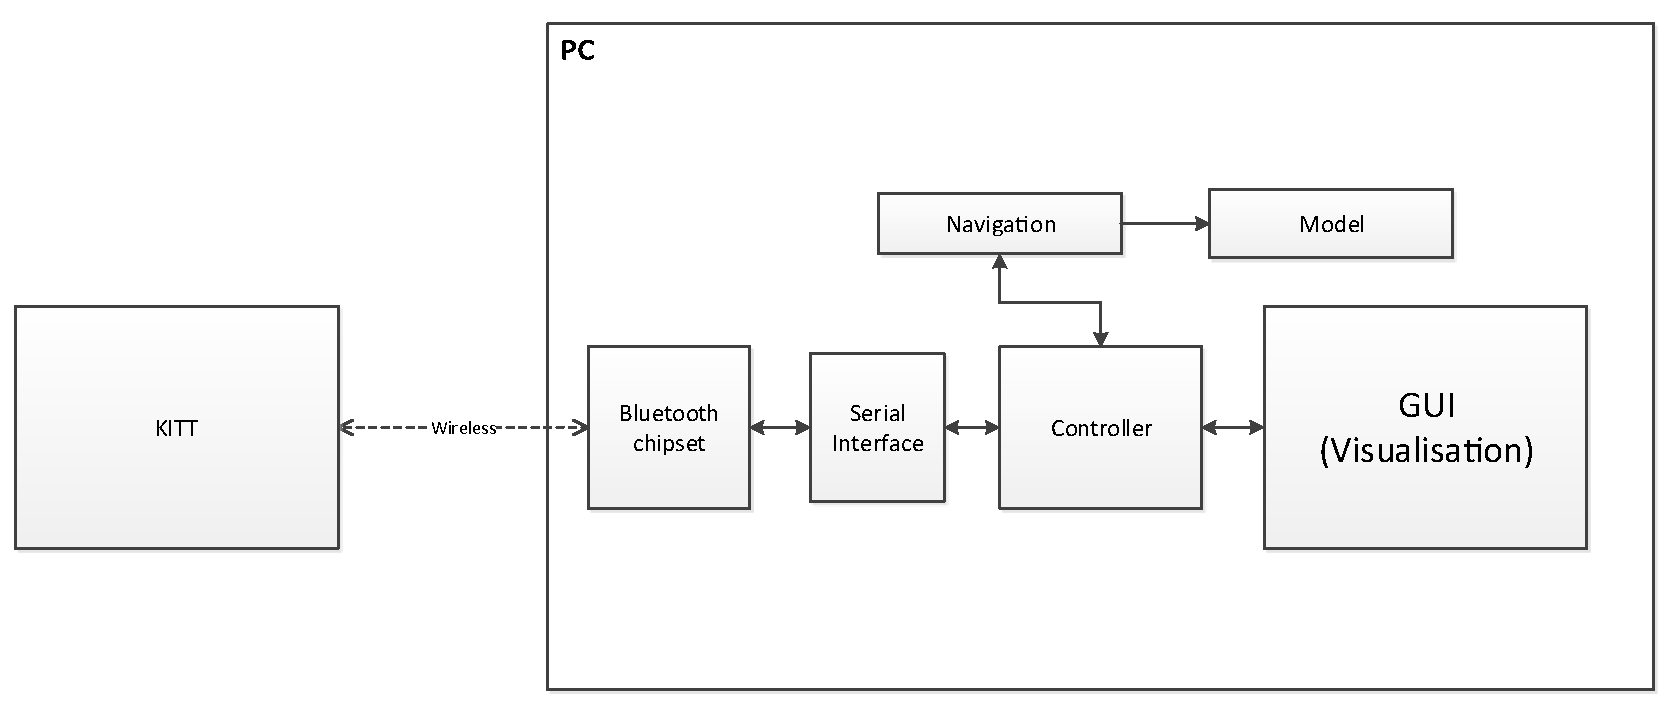
\includegraphics[width=\textwidth]{resources/system-diagram.pdf}
    	\caption{The system in diagram form}
    	\label{fig:system-diagram}
\end{figure}
Here follows a rundown of all the components.
\section{GUI (Visualization)}
This part handles everything to do with the GUI and the Databindingsa to the underlying parts.
The associated classes and files are:
\begin{itemize}
\item App (Appendix listing \ref{lst:Director-App.xaml.cs} \& \ref{lst:Director-App.xaml})
\item MainWindow (Appendix listing \ref{lst:Director-MainWindow.xaml.cs} \& \ref{lst:Director-MainWindow.xaml})
\item Data (Appendix listing \ref{lst:Director-Data.cs})
\item Arrow (Appendix listing \ref{lst:Director-Arrow.cs})
\item Visualization (Appendix listing \ref{lst:Director-Visualization.cs})
\item Databindings (Appendix listing \ref{lst:Director-Databindings.cs})
\end{itemize}
\section{Controller}
This part is the "brain", here the serial events are handled and commands sent.
The associated classes and files are:
\begin{itemize}
\item Controller (Appendix listing \ref{lst:Director-Controller.cs})
\item Data (Appendix listing \ref{lst:Director-Data.cs})
\end{itemize}
\section{Navigation}
This is not yet in use. Now the Target field on the Controller class serves this function.
The associated classes, interfaces and files are:
\begin{itemize}
\item StandardNavigation (Appendix listing \ref{lst:Director-StandardNavigation.cs})
\item INavigator (Appendix listing \ref{lst:Director-INavigator.cs})
\end{itemize}
\section{Observer}
This part is the gateway to the implemented model.
The associated classes and files are:
\begin{itemize}
\item Observer (Appendix listing \ref{lst:Director-Observer.cs})
\end{itemize}
\section{Model}
This part constsist of a standarized interface and a couple of implemented models.
Those are drop-in replacements of each other.
Our currently used model is PDEpicModel.
The associated classes, interfaces and files are:
\begin{itemize}
\item IModel (Appendix listing \ref{lst:Director-IModel.cs})
\item PDEpicModel (Appendix listing \ref{lst:Director-PDEpicModel.cs})
\item PDDefaultModel (Appendix listing \ref{lst:Director-PDDefaultModel.cs})
\item PIDModel (Appendix listing \ref{lst:Director-PIDModel.cs})
\end{itemize}
\section{Serial}
This part handles all serial communication asynchronously and drives the receive events.
The associated classes, interfaces and files are:
\begin{itemize}
\item ISerial (Appendix listing \ref{lst:Communication-ISerial.cs})
\item SerialDataEvent (Appendix listing \ref{lst:Communication-SerialDataEvent.cs})
\item SerialInterface (Appendix listing \ref{lst:Communication-SerialInterface.cs})
\end{itemize}
\section{Bluetooth Chipset}
The adapter we use most of the time is an Intel(R) Centrino(R) Wireless Bluetooth(R) 4.0 + High Speed Adapter embedded together with the WiFi module in one of our own laptops.

\section{Systen response}
In figure \ref{fig:system-response} you can see the data of a run towards the wall.
\begin{figure}[H]
	\centering
    	\setlength\figureheight{4cm}
    	\setlength\figurewidth{0.8\linewidth}
    	% This file was created by matlab2tikz v0.4.6 running on MATLAB 8.3.
% Copyright (c) 2008--2014, Nico Schlömer <nico.schloemer@gmail.com>
% All rights reserved.
% Minimal pgfplots version: 1.3
% 
% The latest updates can be retrieved from
%   http://www.mathworks.com/matlabcentral/fileexchange/22022-matlab2tikz
% where you can also make suggestions and rate matlab2tikz.
% 
\begin{tikzpicture}

\begin{axis}[%
width=\figurewidth,
height=\figureheight,
scale only axis,
xmin=0,
xmax=4.5,
xlabel={t (s)},
ymin=-20,
ymax=310,
ylabel={x (cm) \& input signal},
legend style={draw=black,fill=white,legend cell align=left}
]
\addplot [color=blue,solid]
  table[row sep=crcr]{
0	300	\\
0.1	300	\\
0.2	300	\\
0.3	300	\\
0.4	300	\\
0.5	300	\\
0.6	301	\\
0.7	288	\\
0.8	288	\\
0.9	274	\\
1	259	\\
1.1	243	\\
1.2	225	\\
1.3	206	\\
1.4	184	\\
1.5	184	\\
1.6	164	\\
1.7	143	\\
1.8	120	\\
1.9	96	\\
2	71	\\
2.1	71	\\
2.2	46	\\
2.3	26	\\
2.4	16	\\
2.5	14	\\
2.6	14	\\
2.7	13	\\
2.8	13	\\
2.9	13	\\
3	13	\\
3.1	13	\\
3.2	13	\\
3.3	14	\\
3.4	14	\\
3.5	14	\\
3.6	15	\\
3.7	15	\\
3.8	14	\\
3.9	14	\\
4	15	\\
4.1	15	\\
4.2	15	\\
4.3	16	\\
4.4	16	\\
4.5	15	\\
};
\addlegendentry{Sensordata Right};

\addplot [color=black!50!green,solid]
  table[row sep=crcr]{
0	300	\\
0.1	301	\\
0.2	301	\\
0.3	300	\\
0.4	300	\\
0.5	300	\\
0.6	304	\\
0.7	292	\\
0.8	292	\\
0.9	279	\\
1	265	\\
1.1	249	\\
1.2	230	\\
1.3	213	\\
1.4	191	\\
1.5	191	\\
1.6	171	\\
1.7	149	\\
1.8	127	\\
1.9	104	\\
2	78	\\
2.1	78	\\
2.2	54	\\
2.3	30	\\
2.4	16	\\
2.5	11	\\
2.6	12	\\
2.7	10	\\
2.8	10	\\
2.9	10	\\
3	10	\\
3.1	10	\\
3.2	10	\\
3.3	11	\\
3.4	11	\\
3.5	11	\\
3.6	12	\\
3.7	12	\\
3.8	12	\\
3.9	11	\\
4	12	\\
4.1	12	\\
4.2	12	\\
4.3	13	\\
4.4	13	\\
4.5	12	\\
};
\addlegendentry{Sensordata Left};

\addplot [color=red,solid]
  table[row sep=crcr]{
0	8	\\
0.1	8	\\
0.2	8	\\
0.3	8	\\
0.4	8	\\
0.5	8	\\
0.6	8	\\
0.7	8	\\
0.8	8	\\
0.9	8	\\
1	8	\\
1.1	8	\\
1.2	8	\\
1.3	8	\\
1.4	8	\\
1.5	8	\\
1.6	8	\\
1.7	0	\\
1.8	6	\\
1.9	-8	\\
2	-10	\\
2.1	-14	\\
2.2	8	\\
2.3	-15	\\
2.4	-15	\\
2.5	0	\\
2.6	0	\\
2.7	0	\\
2.8	-9	\\
2.9	0	\\
3	0	\\
3.1	-8	\\
3.2	0	\\
3.3	0	\\
3.4	0	\\
3.5	-7	\\
3.6	0	\\
3.7	0	\\
3.8	-7	\\
3.9	0	\\
4	0	\\
4.1	0	\\
4.2	-7	\\
4.3	0	\\
4.4	0	\\
4.5	-7	\\
};
\addlegendentry{Input signals};

\end{axis}

\begin{axis}[%
width=\figurewidth,
height=\figureheight,
scale only axis,
xmin=0,
xmax=1,
ymin=0,
ymax=1,
hide axis,
axis x line*=bottom,
axis y line*=left
]
\addplot [color=black,solid,line width=0.0pt,mark=square*,mark options={solid,fill=black,draw=white},forget plot]
  table[row sep=crcr]{
0.5	0.989690721649485	\\
};
\addplot [color=black,solid,line width=0.0pt,mark=square*,mark options={solid,fill=black,draw=white},forget plot]
  table[row sep=crcr]{
0.992175273865415	0.5	\\
};
\addplot [color=black,solid,line width=0.0pt,mark=square*,mark options={solid,fill=black,draw=white},forget plot]
  table[row sep=crcr]{
0.5	0.0103092783505155	\\
};
\addplot [color=black,solid,line width=0.0pt,mark=square*,mark options={solid,fill=black,draw=white},forget plot]
  table[row sep=crcr]{
0.00782472613458529	0.5	\\
};
\addplot [color=black,solid,line width=0.0pt,mark=square*,mark options={solid,fill=black,draw=white},forget plot]
  table[row sep=crcr]{
0.00782472613458529	0.989690721649485	\\
};
\addplot [color=black,solid,line width=0.0pt,mark=square*,mark options={solid,fill=black,draw=white},forget plot]
  table[row sep=crcr]{
0.992175273865415	0.0103092783505155	\\
};
\addplot [color=black,solid,line width=0.0pt,mark=square*,mark options={solid,fill=black,draw=white},forget plot]
  table[row sep=crcr]{
0.992175273865415	0.989690721649485	\\
};
\addplot [color=black,solid,line width=0.0pt,mark=square*,mark options={solid,fill=black,draw=white},forget plot]
  table[row sep=crcr]{
0.00782472613458529	0.0103092783505155	\\
};
\end{axis}
\end{tikzpicture}%    	
    	\caption{The system response of the “drive-to-wall command”.}
    	\label{fig:system-response}
\end{figure}

\end{document}